% Graphic for TeX using PGF
% Title: /home/enberg/Diagram1.dia
% Creator: Dia v0.97.2
% CreationDate: Mon Apr 28 21:21:06 2014
% For: enberg
% \usepackage{tikz}
% The following commands are not supported in PSTricks at present
% We define them conditionally, so when they are implemented,
% this pgf file will use them.
\ifx\du\undefined
  \newlength{\du}
\fi
\setlength{\du}{15\unitlength}
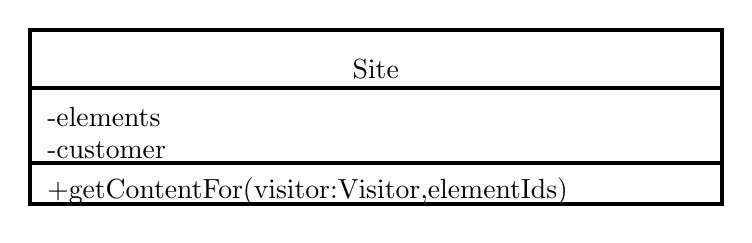
\begin{tikzpicture}
\pgftransformxscale{1.000000}
\pgftransformyscale{-1.000000}
\definecolor{dialinecolor}{rgb}{0.000000, 0.000000, 0.000000}
\pgfsetstrokecolor{dialinecolor}
\definecolor{dialinecolor}{rgb}{1.000000, 1.000000, 1.000000}
\pgfsetfillcolor{dialinecolor}
\pgfsetlinewidth{0.100000\du}
\pgfsetdash{}{0pt}
\definecolor{dialinecolor}{rgb}{1.000000, 1.000000, 1.000000}
\pgfsetfillcolor{dialinecolor}
\fill (15.300000\du,-6.800000\du)--(15.300000\du,-5.400000\du)--(31.970000\du,-5.400000\du)--(31.970000\du,-6.800000\du)--cycle;
\definecolor{dialinecolor}{rgb}{0.000000, 0.000000, 0.000000}
\pgfsetstrokecolor{dialinecolor}
\draw (15.300000\du,-6.800000\du)--(15.300000\du,-5.400000\du)--(31.970000\du,-5.400000\du)--(31.970000\du,-6.800000\du)--cycle;
% setfont left to latex
\definecolor{dialinecolor}{rgb}{0.000000, 0.000000, 0.000000}
\pgfsetstrokecolor{dialinecolor}
\node at (23.635000\du,-5.850000\du){Site};
\definecolor{dialinecolor}{rgb}{1.000000, 1.000000, 1.000000}
\pgfsetfillcolor{dialinecolor}
\fill (15.300000\du,-5.400000\du)--(15.300000\du,-3.600000\du)--(31.970000\du,-3.600000\du)--(31.970000\du,-5.400000\du)--cycle;
\definecolor{dialinecolor}{rgb}{0.000000, 0.000000, 0.000000}
\pgfsetstrokecolor{dialinecolor}
\draw (15.300000\du,-5.400000\du)--(15.300000\du,-3.600000\du)--(31.970000\du,-3.600000\du)--(31.970000\du,-5.400000\du)--cycle;
% setfont left to latex
\definecolor{dialinecolor}{rgb}{0.000000, 0.000000, 0.000000}
\pgfsetstrokecolor{dialinecolor}
\node[anchor=west] at (15.450000\du,-4.700000\du){-elements};
% setfont left to latex
\definecolor{dialinecolor}{rgb}{0.000000, 0.000000, 0.000000}
\pgfsetstrokecolor{dialinecolor}
\node[anchor=west] at (15.450000\du,-3.900000\du){-customer};
\definecolor{dialinecolor}{rgb}{1.000000, 1.000000, 1.000000}
\pgfsetfillcolor{dialinecolor}
\fill (15.300000\du,-3.600000\du)--(15.300000\du,-2.600000\du)--(31.970000\du,-2.600000\du)--(31.970000\du,-3.600000\du)--cycle;
\definecolor{dialinecolor}{rgb}{0.000000, 0.000000, 0.000000}
\pgfsetstrokecolor{dialinecolor}
\draw (15.300000\du,-3.600000\du)--(15.300000\du,-2.600000\du)--(31.970000\du,-2.600000\du)--(31.970000\du,-3.600000\du)--cycle;
% setfont left to latex
\definecolor{dialinecolor}{rgb}{0.000000, 0.000000, 0.000000}
\pgfsetstrokecolor{dialinecolor}
\node[anchor=west] at (15.450000\du,-2.900000\du){+getContentFor(visitor:Visitor,elementIds)};
\label{Content objektet}
\end{tikzpicture}
